\chapter{An algorithm for testing pattern-avoidance of a general pattern}
We begin with a very basic algorithm that we improve a lot to get a fast algorithm for testing avoidance of a general pattern.

\section{Sketch of a brute force algorithm}
Let $L=\{l_1,l_2,\cdots,l_{w+h}\}$ be the lines (rows and columns) of the pattern $P$. Partial mapping of lines of $P$ is a function $f$ from $L'\subseteq L$ to lines of the big matrix $M$ satisfying two conditions: 
%The basic algorithm we use goes as follows. It takes a line $l$ (row or column) of the pattern and for each line $L$ of the big matrix it decides whether the pattern can be mapped there. It can, if three conditions are all met at once:
\begin{itemize}
%\item Both $l$ and $L$ are rows or they are both columns.
%\item If $l'$ is a line of $P$ parallel to $l$ that has been mapped previously to line $L'$, we want $l<l'\Leftrightarrow L<L'$. This means we want the mapped lines to be in the same order as they were in the pattern.
%\item If $l'$ is a line of the pattern orthogonal to $l$ that has been mapped previously to line $L'$ and there is a one-entry at the intersection of $l$ and $l'$, there has to be one-entry at the intersection of $L$ and $L'$.
\item Both $l'\in L'$ and $f(l')$ are rows or they are both columns.
\item If $l'\in L'$ and $l''\in L'$ are both rows or columns and $l'<l''$, then $f(l')<f(l'')$. This means partial mapping keeps the order of the lines.
\item If $l'\in L'$ is a row of $P$ and $l''\in L'$ is a column of $P$ and there is a one-entry at the intersection of $l'$ and $l''$, then there is a one-entry at the intersection of $f(l')$ and $f(l'')$.
\end{itemize}
The basic algorithm we use goes as follows. First it maps $l_1$ to all possible lines of $M$, creating partial mappings of $\{l_1\}\subseteq L$. For $k=2,\cdots,w+h$ it takes each partial mapping from previous iteration and extends it by adding line $l_k$ to the partial mapping in all possible ways. If we manage to map all the lines of $P$, then $M$ does not avoid it and if at some point there are no partial mappings to extend it means $M$ avoids $P$.

Note that we do not use even the slightest heuristics like not to map a line having $k$ one-entries to a line with fewer one-entries. The fact we made a useless mapping will be discovered at the time we try to map the $k$-th orthogonal line (or maybe earlier). This leads to possibly very large number of partial mappings and our next goal will be to reduce this number significantly.

\section{Equivalent mappings}
There are a lot of possible heuristics we can check before adding a line to a partial mapping, but the most fundamental operation we do to decrease the number of found mapping is saying that two mapping are equivalent.

The idea behind it is very basic. There is no need to remember two different mappings if they can be both extended exactly the same way as our function is only supposed to check whether a pattern can be mapped to a big matrix not to find all such mappings.

A \textbf{level} of a partial mapping is the number of lines mapped by the mapping.

We call a line $l$ of a pattern \textbf{important} in a partial mapping if one of the conditions is met:
\begin{itemize}
\item An adjacent line of the pattern has not been mapped yet.
\item There is a one-entry on the line $l$ at the intersection with line $l'$ that has not been mapped yet.
\end{itemize}.
Otherwise the line is \textbf{unimportant} in the mapping.

At the beginning, when no line is mapped, all lines are important. After some lines get mapped a line can become unimportant in the partial mapping as all lines that bound in are in the mapping as well. If a line is unimportant in a partial mapping of some level, it will stay unimportant in all extensions of the mapping we can find.

We say two partial mappings of the same level are \textbf{equivalent} if all important lines in the mapping of that level are mapped to the same lines of the big matrix in both mappings.

\centerline{\mbox{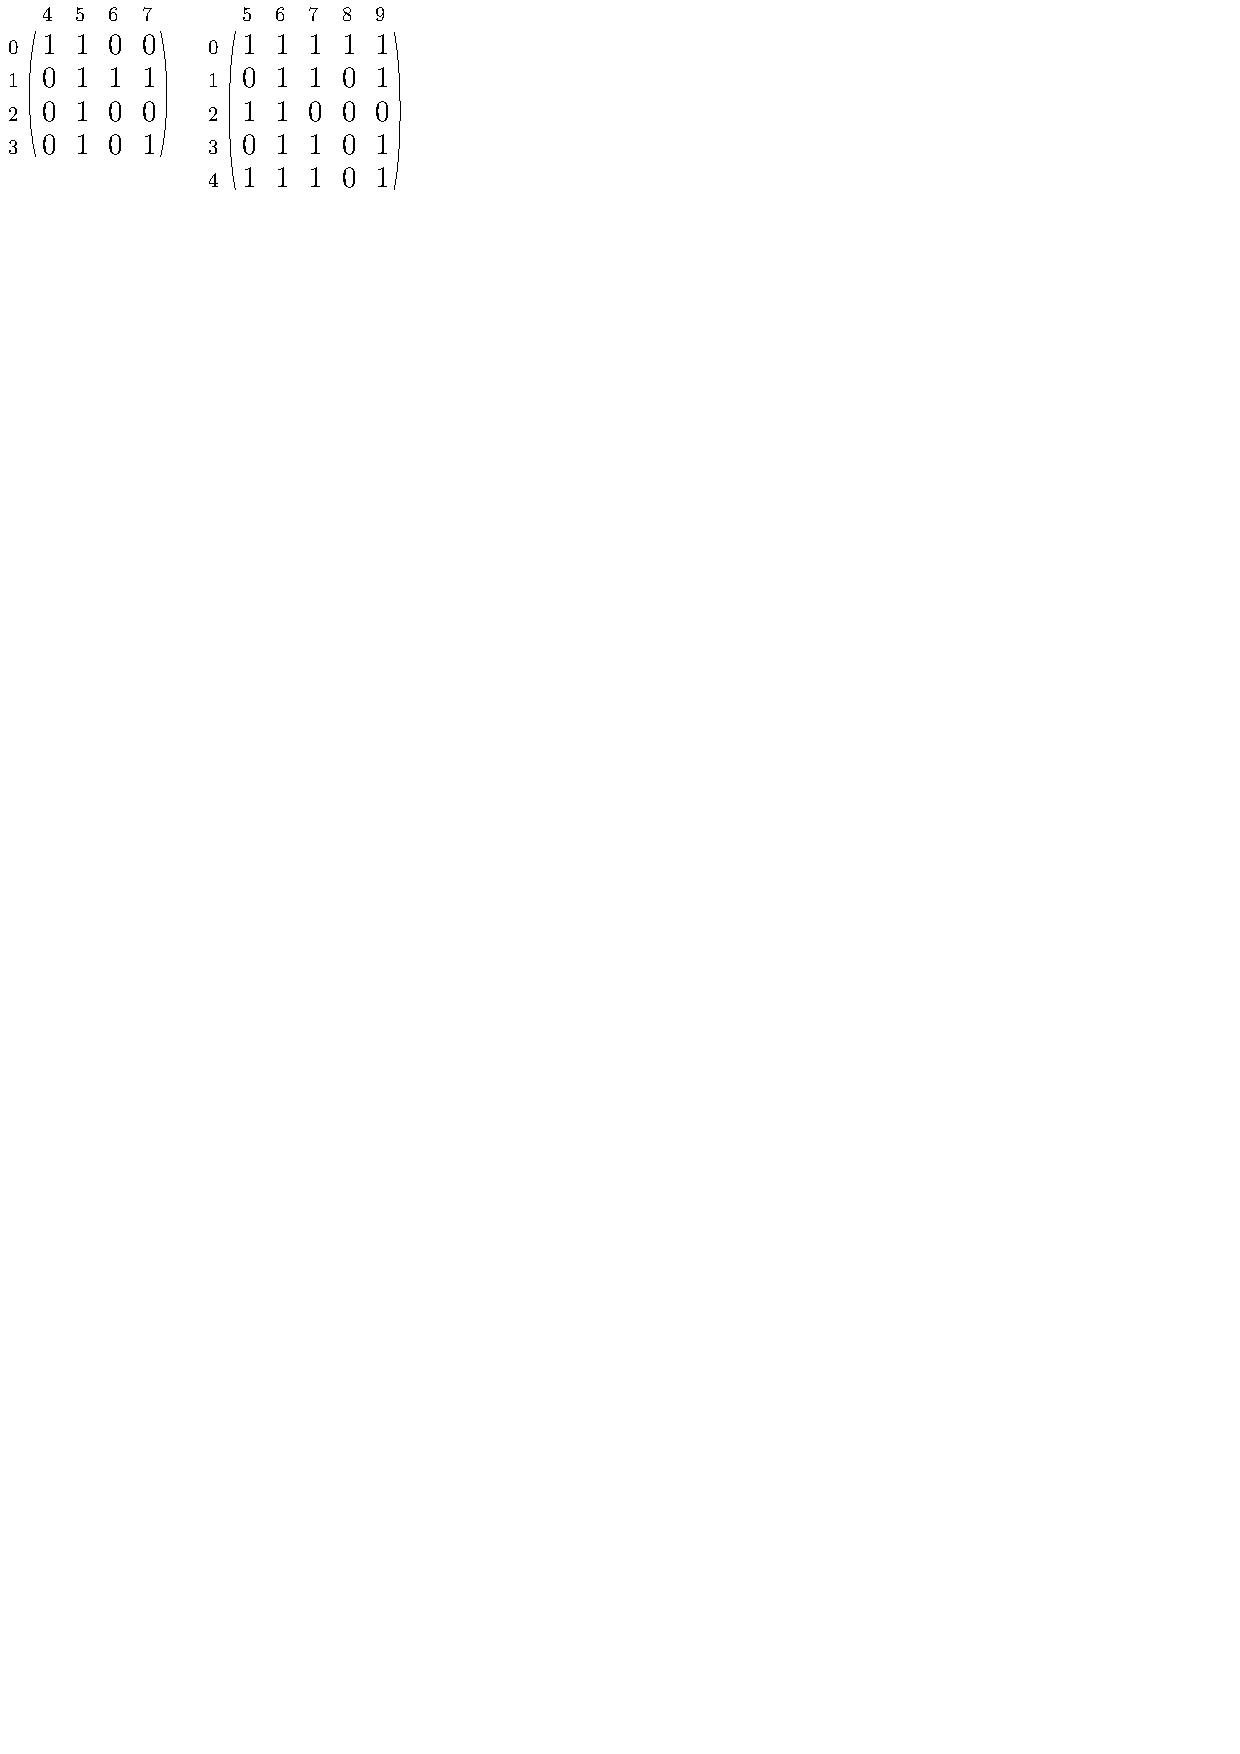
\includegraphics[width=100mm]{../img/equivalent.pdf}}}
For $P$ being the left matrix of the picture and $M$ being the other matrix in the picture, in partial mapping $f=\{(1,1),(2,2),(3,4),(5,6)\}$ line $2$ is unimportant, as both lines $1$ and $3$ are mapped and so is line $5$ - the only line to intersect line $2$ in a one-entry. Line $3$ is important, because there is line $7$ intersecting it in one-entry, which is not mapped.

In the same situation as above, consider a different partial mapping $f'=\{(1,1),(2,3),(3,4),(5,6)\}$, which is a mapping of the same level as $f$ and only differs from $f$ in mapping line $2$. The line $2$ is unimportant and by the definition of equivalent partial mappings, $f$ and $f'$ are equivalent. The idea behind this notion is simple. It is not important where we map line $2$, because it does not restrict where we can map other line that have not been mapped yet. This means that if a partial mapping $f$ can be somehow extended, the equivalent partial mapping $f'$ can be extended in the same way; therefore, it is sufficient to only extend one of them in order to find one full mapping. Note that it would be also sufficient to only extend one of the partial mappings if we were looking for all full mappings, but we would need to keep the information about unimportant lines.